\documentclass{article}
\usepackage[utf8]{inputenc}
\usepackage{macros}

\title{Densest low-rank subgraph}
\author{Vasily}
\date{May 2020}

\begin{document}

\maketitle

\section{Introduction}
\subsection{Definitions and Notation}
\begin{definition}
Let $G = (V,E)$ be a graph. For $S\subset V$ we define $E(S)$ to be the set of edges induced by $S$. We will call $\rho(S) = \frac{|E(S)|}{|S|}$ the density of $S$.
\end{definition}

\begin{definition}
Let $S\subset V\subset \R^d$ and $k\geq 1$ an integer, and $X$ be a matrix, whose columns are given by $V$. We define $A_S$ to be the matrix with columns given by $S$, and
\begin{equation}\label{eqn: L2 objective, not normalized}
    e_k(S) = \norm{A_S - A_{S,k}}^2 = \sum_{i=k+1}^{\rank A_S} \sigma_i^2
\end{equation}
to be the error of $S$, where $A_{S,k}$ is the best $k$-rank approximation of $A_S$, and $\sigma_i$ is the
$i$\textsuperscript{th} largest principal value. If $E\subset \R^d$ is the set of (left) principal vectors of $A_k$, and $e_k(S) \leq M$ for some $M$, we say that $E$ $M$-spans $S$. Note that if $M=0$, then $E$ simply spans $S$.

Additionally, let
\begin{equation}\label{eqn: L2 objective, normalized}
    e'_k(S) = \norm{A_S - A_{S,k}}^2/\norm{A_S}^2 = \frac{\sum_{i\geq k+1} \sigma_i^2}{\sum_{i\geq 1} \sigma_i^2}
\end{equation}
\end{definition}
Letting $\set{v_1,\dots,v_N} = V$ we have $A_S = X D$, where $D$ is a diagonal matrix with $D_{i,i} = 1$ whenever $v_i \in S$.

\subsection{Useful facts about SVD}
Let $A$ be a $d\times n$ matrix of rank $r$ with columns being points in $\R^d$. The SVD of $A$ is
$$\sum_{i\leq r}\sigma_i u_i v_i^T = U \Sigma V^T.$$
Vectors $u_i$ are the (left) singular vectors of $A$ with the property
$$u_i = \arg \max_{\norm{u_i}=1, u_i \perp u_1\dots u_{i-1}}\norm{A u_i},$$
where $\norm{A u_i} = \sigma_i$ is sum of squares of lengths of projections of points onto $u_i$.

The relationship between the Frobenius norm and the singular values is
$$\norm{A}^2 = \sum_{i,j}a_{i,j}^2 = \sum \sigma_i^2.$$
Given $A_k = \sum_{i\leq k}\sigma_i u_i v_i^T$, the best $k$-rank approximation of $A$ in both the 2-norm and the Frobenius norm,
$$\norm{A - A_k}^2 = \norm{\sum_{i}\sigma_i u_i v_i^T - \sum_{i\leq k}\sigma_i u_i v_i^T}^2 = \norm{\sum_{i > k}\sigma_i u_i v_i^T}^2 = \sum_{i>k}\sigma_i^2.$$
Thus, $$e_k(S) = \sum_{i>k}\sigma_i^2 = \text{ sum of squared lengths of residues from projecing onto the first $k$ singular vectors},$$ where $\sigma_i$ are the singular values of $S$ viewed as a matrix. This gives an algebraic and a geometric way to interpret the error.

\subsection{Questions}
For the questions below, $n > k \geq 1$ are integers and $G = (V,E)$ is a graph with $V\subset \R^d$. We have four related objectives.
\begin{align}
    F(S) &= \max_{S \subset V} \lambda \rho(S) - e_k(S)\label{eqn: n not given, not normalized}\\
    F(S) &= \max_{S \subset V, |S| = n} \lambda \rho(S) - e_k(S)\label{eqn: n given, not normalized}\\
    F(S) &= \max_{S \subset V} \lambda \rho(S) - e'_k(S)\label{eqn: n not given, normalized}\\
    F(S) &= \max_{S \subset V, |S| = n} \lambda \rho(S) - e'_k(S)\label{eqn: n given, normalized}
\end{align}

Note that the unnormalized objective \ref{eqn: L2 objective, not normalized} is biased towards choosing vectors of low norm. Thus, objective \ref{eqn: L2 objective, normalized} might be preferred.
 Additionally, note that if there exists an algorithm for \ref{eqn: n given, normalized}, then by repeating it $N$ times, problem \ref{eqn: n not given, normalized} can be solved. Thus, we focus on problem \ref{eqn: n given, normalized}.

\begin{question}[Forgetting about density]\label{problem: no density}
    Find subset of vertices $S\subset V$ of size $n$ that minimizes $e_k(S)$. The binary version of the problem is: ``\textit{Given $M \geq 0$ and integers $k,n\geq 1$, does there exists  $S\subset V$ of size $n$ such that $e_k(S)\leq M$?}" Is this problem \textbf{NP}-hard?
\end{question}

\begin{proof}[Answer]
Case $M=0$ is not \textbf{NP}-hard for any given $k$, by algorithm \ref{alg: enumerative with M = 0}, but the runnning time is exponential in $k$. Also, if the dimension $m$ is fixed, the problem is not \textbf{NP}-hard by \ref{subsection: our problem is in P}.
\end{proof}

\subsection{Relationship between constrained and unconstrained objectives}
For objectives \ref{eqn: n not given, not normalized} and \ref{eqn: n not given, normalized} with parameter $n$ not given, it is interesting to contemplate how many nodes will be in the optimal solution. Letting $n^*$ be the number of nodes in the set with the highest density $E(S)/|S|$,
if $n^* \leq k$, then, clearly, the number of nodes in the optimal solution to problems \ref{eqn: n not given, not normalized} and \ref{eqn: n not given, normalized} is $n^*$. Otherwise, the optimal solution contains from $k$ to $n^*$ nodes, depending on the data and on $\lambda$.

\subsection{Varying $\lambda$}
If $\lambda = 0$, the problem reduces to only dealing with the algebraic structure of the problem. If $\lambda = \infty$, the problem reduces to finding the densest subgraph. What happens when $\lambda$ is some intermediate value? And how to select $\lambda$ in practice?

\section{Ideas}
\subsection{Connection with MCD}
The MCD problem from \cite{bernholt2004complexity} is related to our problem in the following algebraic way. For a given set $S$ and the matrix it spans (call it $S$ too), its SVD is given by $S = U \Sigma V^T$, where $SS^T = U \Sigma^2 U^T$ is the covariance matrix. Thus, the objective function in MCD is $$\det{S} = \det{SS^T} = \det{U \Sigma^2 U^T} = \det{\Sigma^2} = \prod_{i}\sigma_i^2 = \text{ product of singular values squared}.$$ The objective function to be minimized in our problem is $$e_k(S) = \sum_{i \geq k+1}\sigma_i^2.$$

\section{Performance Evaluation}
\begin{figure}[H]\label{img: FastLowRank performance}
    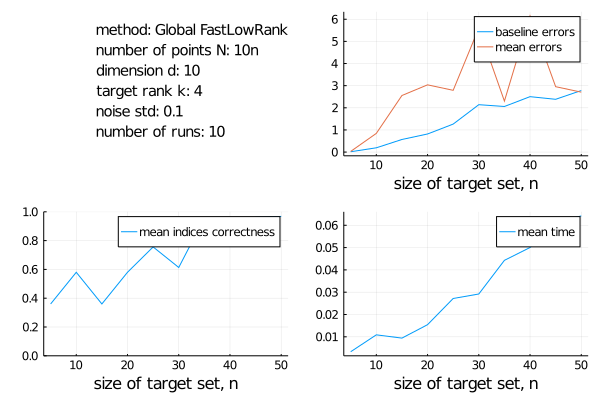
\includegraphics[width = 0.8\textwidth]{images/GlobalFastLowRank.png}
    \caption{GlobalFastLowRank performance}
    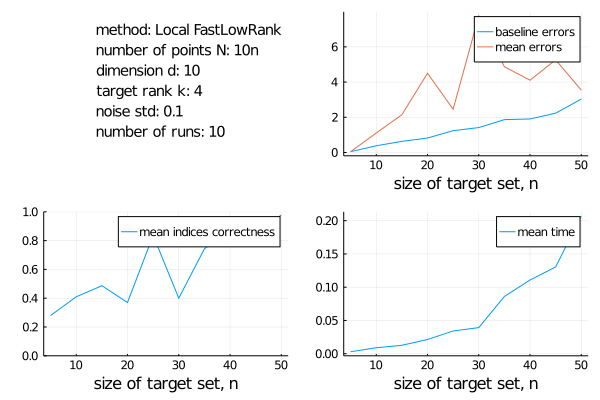
\includegraphics[width = 0.8\textwidth]{images/LocalFastLowRank.png}
    \caption{LocalFastLowRank performance}
\end{figure}


\printbibliography

\section{Appendix}
\subsection{naive algorithms}
\begin{proof}[Answer to \ref{problem: no density}]
Consider the following algorithm that returns $S$ if exists $S$ with $e_k(S) = 0$, and ``false" otherwise:
\begin{algorithm}[H]
      \caption{}\label{alg: enumerative with M = 0}
    \begin{algorithmic}[1]
    \Procedure{FindS}{V,n,k}
    \For{each set $\set{e_1,...,e_k}\subset V$ of size $k$}:
        \State $M = \Big(e_1,...,e_k\Big)$
        \State $S = E$
        \For{$v\in V\setminus \set{e_1,...,e_k}$}
            \If{$Mx = v$ has a solution}\label{line: direct Alg, check span}
                \State $S = S\cup \set{v}$
            \EndIf
        \EndFor
        \If{$|S|\geq n$}
            \State \textbf{return} $S$
        \EndIf
    \EndFor
    \State \textbf{return} false
    \EndProcedure
    \end{algorithmic}
\end{algorithm}

Note that line \ref{line: direct Alg, check span} checks if $v\in \vspan{\set{e_1,...,e_k}}$, and takes time $\Theta(m^2k)$ or $\Theta(mk)$ if a (LUP or any other) factorization of $M$ is precomputed. The overall complexity of algorithm \ref{alg: enumerative with M = 0} is $O(\binom{N}{k}Nkm)$ (by precomputing a factorization of $M$ to make solving $Mx=v$ faster), where $N = |V|$. For small $k<<N$ and $m = O((k-1)!)$ the complexity is $O(N^{k+1})$.

It is not immediately clear that the algorithm is correct. For a set $S\subset V$ $e_k(S)=0$ is equivalent to $S$ being spanned by $k$ vectors. If such $S$ does not exist, the algorithm will not find one. If such $S$ exists, there are $k$ vectors that span $S$. So $d := \dim \vspan{S} \leq k$. So there exist $d$ vectors in $S$ that span $S$. Thus the $k$ vectors can be chosen from $S$, and the algorithm will find them by checking all subsets of $V$ of size $k$.

Now consider the following modification of algorithm \ref{alg: enumerative with M = 0}, which attempts to find $S$ that minimizes $e_k(S)$.

\begin{algorithm}[H]
      \caption{}\label{alg: enumerative with M > 0}
    \begin{algorithmic}[1]
    \Procedure{FindS}{V,n,k}
    \For{each set $E = \set{e_1,...,e_k}\subset V$ of size $k$}:
        \State $M = \Big(e_1,...,e_k\Big)$
        \State $D = $ empty array
        \For{$v\in V\setminus \set{e_1,...,e_k}$}
            \State $x=$ solution to $M^TMx = M^Tv$ (so $x=\proj_{\vspan E}(v)$)
            \State append $\norm{v-Mx}^2$ to $D$
        \EndFor
        \State $S_E = E\cup$ the $n-k$ smallest values of $D$
        \State $e_E = $ sum of $n-k$ smallest values of $D$
    \EndFor
    \State \textbf{return} $S_E$ with smallest $e_E$.
    \EndProcedure
    \end{algorithmic}
\end{algorithm}
Algorithm \ref{alg: enumerative with M > 0} is a simple modification of algorithm \ref{alg: enumerative with M = 0}. On line 6, instead of solving the linear system $Mx = v$ exactly, we find the closest point $x$ in the span of $\set{e_1,...,e_k}$ (which is the projection of $v$ onto $\vspan{\set{e_1,...,e_k}}$), and record the square of distance from $x$ to $v$.

Note that this algorithm is not exact, as opposed to algorithm \ref{alg: enumerative with M = 0}. This is because there might exist a set $\set{e_1,...,e_k}$ that $M-$spans (has error $\leq M$) a set $S$, with $\set{e_1,...,e_k}$ not being a subset of $V$. To be explicit, consider $V=\set{(-1,2),(1,2)}$, $n=2$, $k=1$, $M = 3$. Then there exists vector $e_1=(0,1)$, for which the error is 2, while if $e_k$ were to be picked from $V$, the error would be 3.2. By \cite{rademacher2005matrix} this algorithm is a 4-approximation if $k=1$ and all vectors in $V$ are of unit length.

Clearly, the runtime of algorithm \ref{alg: enumerative with M > 0} is the same as algorithm \ref{alg: enumerative with M = 0}, and is equal to $O(N^{k+1})$, where $N = |V|$.
\end{proof}

\subsection{Our problem is in \textbf{P}}\label{subsection: our problem is in P}
\cite{chawla2013k} notes that a set solving k-means-- for $k=1$ is selectable by a sphere. Similarly, a set solving out problem is selectable by a cylinder for $k=1$. For an arbitrary $k$, a set solving our problem is selectable by a the quadric that describes the points $r$ away from some subspace $E$.

To be precise, let $e_1,\dots,e_k$ be an orthonormal basis for the subset $E$ that solves out problem. Then set $S$ that solves our problem consists of $n$ points closest to $E$. Then exists quadric $Q$ that selects $S$, i.e. exist coefficients $a_i, a_{i,j}$ for $1\leq i\leq j\leq m$ s.t. $A_{i,j} = a_{i,j}$ is a symmetric matrix, and $b_i = a_i$ is a column vector, and for all points in $S$, $x^TAx + x^Tb + a_0 \leq 0$ and for all points not in $S$, $x^TAx + x^Tb + a_0 > 0$.

Let's compute this quadric. Let $r>0$ be the cut-off distance, i.e. $n$ closest points lie within $r$ of $E$, and all other points lie further than $r$ from $E$. Then a quadric selecting $S$ is given by $\norm{x - \proj_{E}(x)}_2^2 - r^2 = 0$. But $\norm{x - \proj_{E}(x)}_2^2 = \norm{x}_2^2 - \norm{\proj_{E}(x)}_2^2$. Note that $\norm{x}_2^2 = \sum_{i=1}^d x_i^2$ and
\begin{align*}
    \norm{\proj_{E}(x)}_2^2 &= \sum_{\ell=1}^k \inp{x}{e_\ell}^2 = \sum_{\ell=1}^k \left(\sum_{i=1}^d x_i e_{\ell,i}\right)^2 = \sum_{\ell=1}^k \left( \sum_{i=1}^d x_i^2 e_{\ell,i}^2 + 2\sum_{1\leq i < j\leq m} x_ix_j e_{\ell,i}e_{\ell,j} \right)\\
    &= \sum_{i=1}^d x_i^2 \left(\sum_{\ell=1}^k  e_{\ell,i}^2\right) + 2\sum_{1\leq i < j\leq m} x_ix_j \left(\sum_{\ell=1}^k  e_{\ell,i}e_{\ell,j} \right)
\end{align*}
So the coefficients for quadric $Q$ are
\begin{align*}
    a_0 &= -r^2,\ a_i = 0 \text{ for $1\leq i\leq m$}\\
    a_{i,i} &= 1 - \left(\sum_{\ell=1}^k  e_{\ell,i}^2 \right) \text{ and } \\
    a_{i,j} &= - \left(\sum_{\ell=1}^k  e_{\ell,i}e_{\ell,j} \right)\text{ for $i\neq j$}.
\end{align*}
Suppose that $V$ is in \textit{general quadric position}, i.e. no hyperplane in $\R^\nu$ contains more than $\nu$ points of $\widehat{\X}$, just like they assume in \cite{bernholt2004complexity}. Then we have an analogue of lemma 2.2. in \cite{bernholt2004complexity}.
\begin{lemma}
Given $V\subset \R^d$ in general quadric position, and a quadric selecting $S\subset V$. Then there exists set $T \subset V$, $|T| = \nu := m(m+3)/2$ such that for the quadric $Q(T)$ the following holds. Let $A,b,a_0$ define $Q(T)$. Then
\begin{align*}
    & x^TAx + x^Tb + a_0 \leq 0,\ x\in S,\\
    & x^TAx + x^Tb + a_0 \geq 0,\ x\in V\setminus S,\\
    & x^TAx + x^Tb + a_0 = 0\ \text{for at most $\nu$ points $x\in V\setminus S$}.
\end{align*}
\end{lemma}
The proof is the same as for lemma 2.2 in \cite{bernholt2004complexity}. Since a set $S$ that solves our problem is selectable by a quadric, the lemma applies, and the algorithm proposed in \cite{bernholt2004complexity} finds $S$ in time $O(N^{\nu+1})$ (the only modification is that instead of selecting a set that gives the smallest covariance determinant, we select a set that has the smallest error of rank-$k$ approximation).

\subsection{FastLowRank (Iterative algorithms)}
\subsubsection{Not normalized}\label{alg: FastLowRank, not normalized}
The following algorithm aims to minimize the non-normalized objective \ref{eqn: L2 objective, not normalized}, i.e. minimize $e_k(S) = \sum_{i\geq k+1}\sigma_i^2$.

Initialize a bunch ($\alpha$) of subsets $S\subset V$. Each $S$ is initialized as follows: first, select $k$ vectors from $V$ u.i.r., and then find $n-k$ points in $V$ that are the closest to the span of the $k$ initial vectors. Now, for each set $S$, compute the set $E = \set{e_1,\dots, e_k}$ of the first $k$ singular vectors, and choose $n$ points from $V$ that are the closest to the span of $E$. Repeat until one of the $\alpha$ trajectories converges. Notice that eventual convergence is guaranteed because at each step the error $e_k(S)$ does not increase.

\subsubsection{Normalized}\label{alg: FastLowRank, normalized}
In order to minimize objective \ref{eqn: L2 objective, normalized}, i.e. minimize $e'_k(S) = \frac{\sum_{i\geq k+1}\sigma_i^2}{\sum_{i\geq 1}\sigma_i^2}$, we need to modify the way we select $S'$. Here is the optimal algorihm for picking $S'$ given $S$.

For each point $x_i$ let $e(x_i) = \sum_{i\geq k+1}\inp{x_i}{u_i}^2$ is the length squared of the residue of $X_i$ ($\set{u_i}$ is the set of left singular vectors of $S$). We aim to find points $S'$, s.t.
 $$\frac{\sum_{i\geq k+1}\sigma_i^2}{\sum_{i\geq 1}\sigma_i^2} = \frac{\sum_{x \in S'}e(x)}{\sum_{x\in S'}\norm{x}^2}$$
 is minimized. Then it suffices to solve the problem of choosing $n$ elements $S'$ out of a subset $\X$ of $\R^2$, lying in the first ocatant, of size $N$, s.t. $$\frac{\sum_{(x,y) \in S'}y}{\sum_{(x,y)\in S'}x} = \text{ slope of }\sum_{(x,y) \in S'}(x,y)$$ is minimized. To do this, note that the point $(x^*,y^*) \in \X$ with the smallest slope must be in $S'$, since the slope of
  $\sum_{(x,y) \in S'}(x,y)$ is a weighted sum of slopes $\set{\frac{y}{x}}_{(x,y)\in S'}$, since $\frac{\sum_{(x,y) \in S'}y}{\sum_{(x,y)\in S'}y} = \frac{\sum_{(x,y) \in S'}x\cdot \frac{y}{x}}{\sum_{(x,y)\in S'}x}$.
  Now, let $\X_1 = \X + (x^*,y^*)/(n-1) = \set{(x,y) + (x^*,y^*)/(n-1): (x,y)\in \X}$, and choose $n-1$ points from $\X_1$ that minimize the slope. This is correct, because the sum of any $n-1$ elements of $\X_1$ is equal to the sum of the corresponding $n-1$ elements of $\X$ plus $(x^*, y^*)$.

  This update step $S \mapsto S'$ is $\Theta(N\cdot n)$, which is $n$ times slower than the equivalent step in the non-normalized version of FastLowRank. With this update step the error does not increase, i.e. $e'_k(S') \leq e'_k(S)$, meaning convergence is guaranteed.

\subsubsection{FastLowRank for graphs}
Since the algorithms above do not take the structure of the graph into account, we need to modify it in order to use it for our problem. At each step we have the set of nodes $S$, and need to pick a new set of nodes $S'$, for which the objective function $F(S') \leq F(S)$ to guarantee convergence.

For a node $v$, let $F(v) = \lambda \deg_S(v) - e_k(v)$, where $\deg_S(v)$ is the degree of $v$ in the subgraph induced by $S$, and $e_k(v) = \sum_{i\geq k+1}\inp{v}{u_i}^2$, where $\set{u_i}$ is the set of left principal vectors of $S$, is the error $v$ contributes to $e(S)$. Here are some ideas for picking $S'$ based on $F(v)$:

\begin{enumerate}
    \item Let $S'$ be $S$ with one node swapped out. The node to swap out is the one with the largest $F(v)$, and the new node to include is the one with the smallest $F(v)$.
    \item Let $S'$ consist of the $n$ points with the lowest $F(v)$. The problem with this approach is that it is not guaranteed that $F(S') \leq F(S)$, although it is likely if the number of triangles in the graph is large. This can be bad if the graph is bipartite or close to it, because there will be no convergence.
    \item Let $F(v) = \lambda d(v) - e_k(v)$, where $d(v) = \sum_{s\in S}\inp{v}{s}$. This brings more linear algebra into the light but it is not clear how relevant this objective is at all.
    \item Pick the core set $C \subset S$ of $n/2$ nodes with highest degrees (or by some other metric) and let $F(v) = \deg_C(v)$. Swap out $n/2$ nodes with lowest $F(v)$.
\end{enumerate}

\subsubsection{Seeding FastLowRank}
The success of FastLowRank depends on a lucky initialization. If a set is initialized close to an optimal set, convergence will be quick, and an optimal set will be recovered. The user shuld be able to give a ``hint'' to FastLowRank by providing one or more partial or complete initializations.




\end{document}
